\section{Methodology} \label{sec:methodology}

\subsection{Granger causality and feedback} \label{sec:granger-causality}
Framework for causality testing was first proposed by Granger \cite{granger69} in 1969.
The original formulation had a general form with an example of a linear autoregressive model provided, further described in \fref{sec:linear-ar}.

Consider two time series $X_t$ and $Y_t$ of length $n$, which are assumed to be weakly stationary.
Lets denote an optimal, least-squares predictor of some time series $X_t$ given another time series $Y_t$ by $P_t(X|Y)$.
The residual errors of the model and its variance are defined as follows: 
$\varepsilon_t(X|Y) = X_t - P_t(X|Y)$ and $\sigma^2(X|Y) = var[\varepsilon_t(X|Y)]$.
Lastly, all available information until time $t$ will be denoted $U_t$.

Given such notation the following definitions are proposed:

\begin{definition} \label{def:causality}
	Causality

	If $\sigma^2(X|U) < \sigma^2(X|U-Y)$, then $Y_t$ causes $X_t$, denoted as $Y_t \Rightarrow X_t$.
\end{definition}
\begin{definition}
	Feedback

	If $\sigma^2(X|U) < \sigma^2(X|U-Y)$ and $\sigma^2(Y|U) < \sigma^2(Y|U-X)$, then there is feedback between $X_t$ and $Y_t$, denoted as $Y_t \Leftrightarrow X_t$.
\end{definition}

The completely unrealistic aspect of the formulation above is having access to the full information $U_t$.
In practice those definitions allow to construct statistical tests and to reason for causal relations between time series.

\subsubsection{Linear autoregressive model} \label{sec:linear-ar}
A simple realization of Granger causality test can be implemented using a two-variable linear autoregressive (AR) model of order $p$.
Two linear predictors of $X_t$ can be constructed as follows:

\begin{equation}
X_t = \sum_{i=1}^{p} \alpha_i X_{t-i} + \varepsilon_{X,t}
\end{equation}
\begin{equation}
X_t = \sum_{i=1}^{p} a_i X_{t-i} + \sum_{i=1}^{p} b_i Y_{t-i} + \varepsilon_{X|Y,t}
\end{equation}
where: $p$ is the order of AR model, $\alpha$, $a$, $b$ are scalar coefficients and $\varepsilon_{X,t}$, $\varepsilon_{X|Y,t}$ are residual errors of the models.
Causal relationship $Y_t \Rightarrow X_t$ can be inferred by comparing variance of residual errors $\varepsilon_{X,t}$ and $\varepsilon_{X|Y,t}$, as stated in \fref{def:causality} in \fref{sec:granger-causality}.

\subsubsection{Diks-Panchenko method}
\cite{diks-panchenko2004}
\cite{hiemstra-jones}
\cite{baek-brock1992}

\subsection{Wavelet transform} \label{sec:wavelet}
The term ``wavelet'' was coined by Grossmann and Morlet \cite{grossmann-morlet}  in the 1980s. 
The theory for this approach was further developed by many researchers, most notably Daubechies \cite{daubechies1990}.

A wavelet can be intuitively understood as a ``short, localized oscillation''.
The so-called mother wavelet, denoted as $\psi(t)$ is a function that satisfies the following conditions:

\begin{equation} \label{eq:wavelet-zero-mean}
	\int\! dt \: \psi (t) = 0
\end{equation}

\begin{equation} \label{eq:wavelet-norm}
	\int\! dt \: |\psi (t)|^2 = 1
\end{equation}
and the \emph{admissability condition}:
\begin{equation}
	\int\! d\omega \: |\omega|^{-1} \left(\mathscr{F} \psi\right)(\omega) < \infty
\end{equation}
where $\left(\mathscr{F} \psi\right)(\omega)$ is the Fourier transform of $\psi(t)$.

This function is then dilated and translated to account for frequency and localization:

\begin{equation}
	\psi^{(a,b)}(t) = \frac{1}{\sqrt{a}} \: \psi\left(\frac{t-b}{a}\right)
\end{equation}
The continuous wavelet transform $W(a,b)$ is a projection of the original signal $x(t)$ on the mother wavelet:

\begin{equation}
	W(a,b) = \int \! dt \: x(t) \psi^{(a,b)}(t)
\end{equation}

There are several widely used wavelet bases, typical examples are: Haar, Morlet, ``Mexican hat'' and Daubechies.
The mother wavelets of those examples are plotted on \fref{fig:wavelets}.

\begin{figure}[h]
	\centering
	\begin{subfigure}{\minipagewidth}
		\centering
		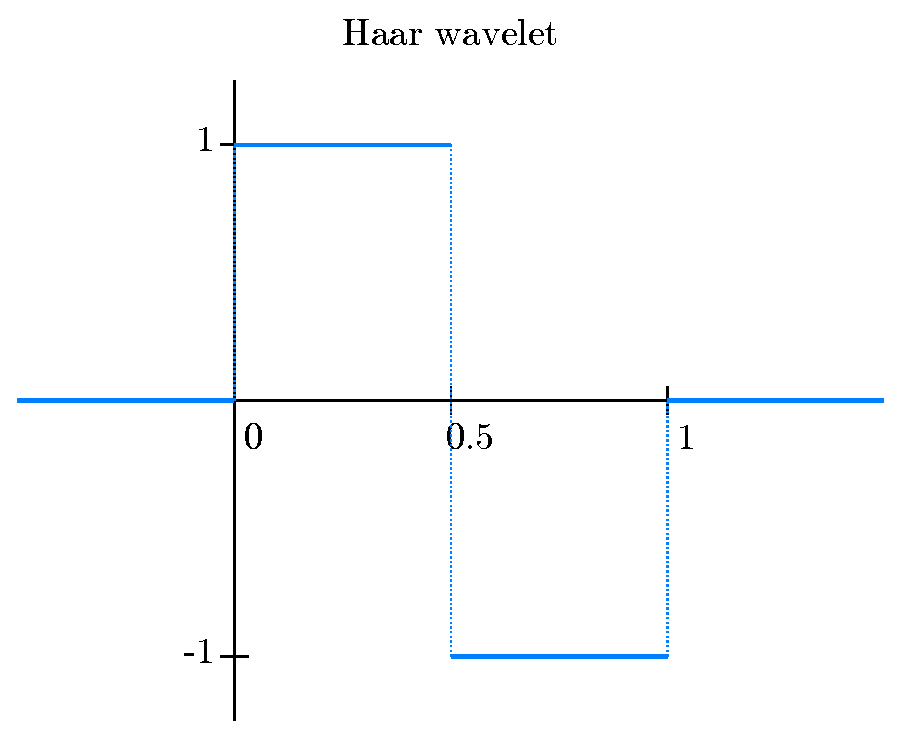
\includegraphics[width=\textwidth]{figures/haar.eps}
		\caption{}
	\end{subfigure}
	\begin{subfigure}{\minipagewidth}
		\centering
		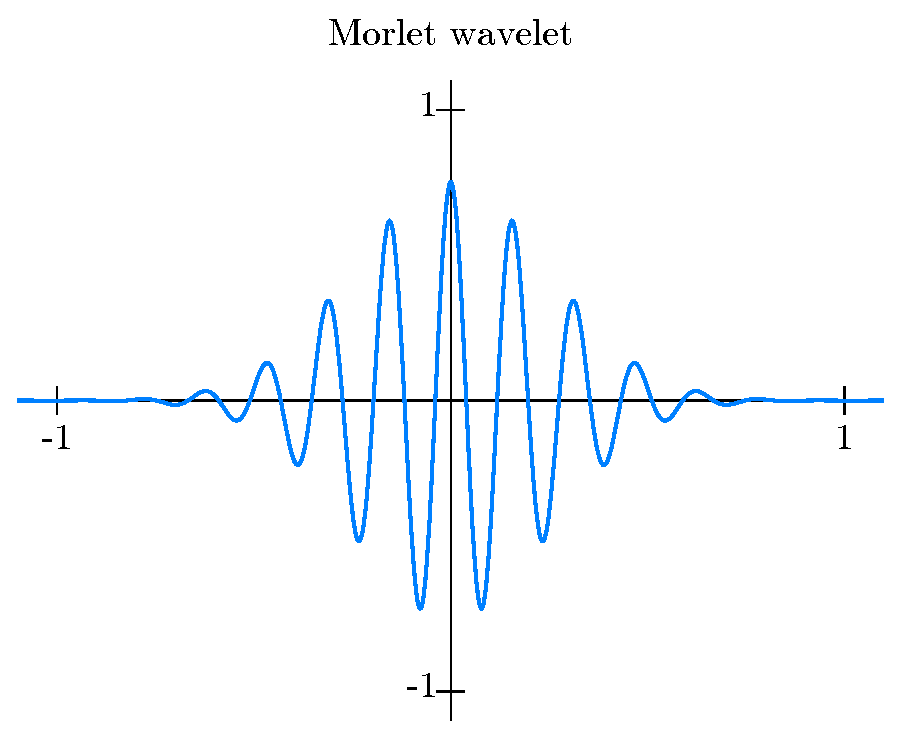
\includegraphics[width=\textwidth]{figures/morlet.eps}
		\caption{}
	\end{subfigure}
	\newline
	\begin{subfigure}{\minipagewidth}
		\centering
		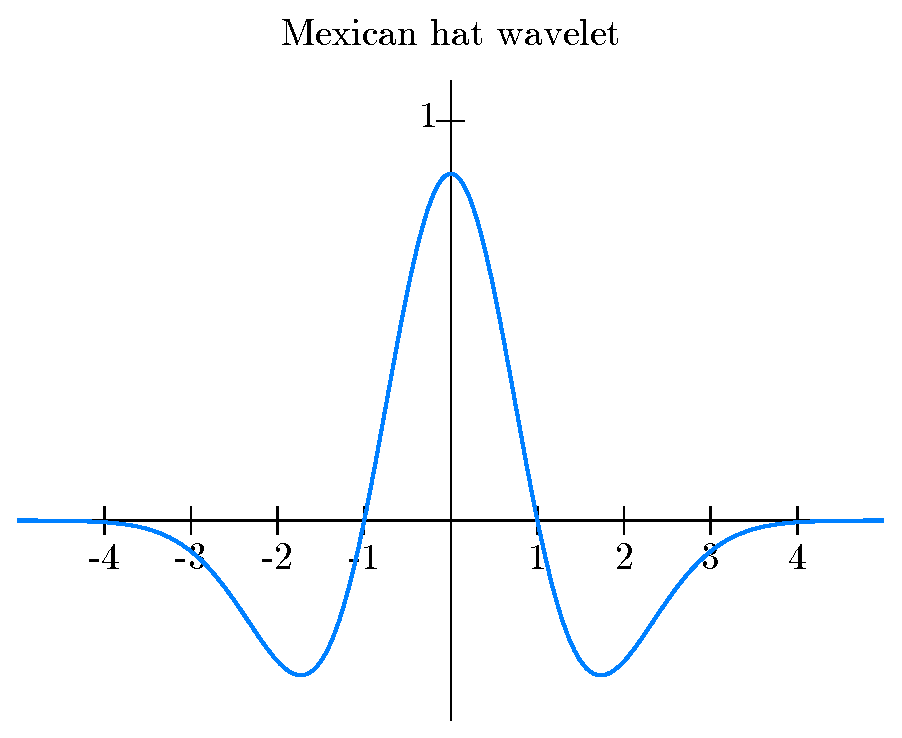
\includegraphics[width=\textwidth]{figures/mexican.eps}
		\caption{}
	\end{subfigure}
	\caption{Mother wavelets of (a) Haar (b) Morlet and (c) Mexican hat.}
	\label{fig:wavelets}
\end{figure}

\subsubsection{Discrete wavelet transform}
For practical purposes, to analyze real-life discrete time series, a discrete wavelet transform (DWT) is used.
It allows to decompose time series into multiple frequency scales.

The DWT is based on two discrete wavelet filters, called \emph{mother wavelet}
(which is a high-pass filter):
\begin{equation}
h_l=(h_0, h_1\ldots h_{L-1})
\end{equation}
and \emph{father wavelet} (a low-pass filter):
\begin{equation}
g_l=(g_0, g_1\ldots g_{L-1}).
\end{equation}
where $L$ is length of the filter.

In the disrete case, conditions \ref{eq:wavelet-zero-mean} and \ref{eq:wavelet-norm} for the mother wavelet become:

\begin{equation}
	\sum_{i=0}^{L-1} h_i = 0
\end{equation}

\begin{equation}
	\sum_{i=0}^{L-1} |h_i|^2 = 1.
\end{equation}
Additionally, $h_l$ is orthogonal to even shifts:

\begin{equation}
	\sum_{i=0}^{L-1} h_i h_{i+2n} = 0
\end{equation}
for all $n \neq 0$.

The father wavelet is constructed from the mother wavelet using the quadrature mirror relation:
\begin{equation}
	g_l = (-1)^{l+1} \:  h_{L-1-l}.
\end{equation}
Moreover, the scaling filter $g_l$ has the following properties:
\begin{center}
\noindent
\begin{minipage}[t]{\minipagewidth}
\begin{equation}
	\sum_{i=0}^{L-1} g_i = \sqrt{2},
\end{equation}
\end{minipage}
\begin{minipage}[t]{\minipagewidth}
\begin{equation}
	\sum_{i=0}^{L-1} |g_i|^2 = 1,
\end{equation}
\end{minipage}

\begin{minipage}[t]{\minipagewidth}
\begin{equation}
	\sum_{i=0}^{L-1} g_i g_{i+2n} = 0,
\end{equation}
\end{minipage}
\begin{minipage}[t]{\minipagewidth}
\begin{equation}
	\sum_{i=0}^{L-1} g_i h_{i+2n} = 0.
\end{equation}
\end{minipage}
\end{center}

In the discrete case dilations and translations of mother wavelet are expressed as:
$a=2^{-j}$ and $b=k 2^{-j}$, where $j, k \in \mathbb{N}$ and $j \leq J = log_2(T)$.
$J$ is the biggest number of scales and $T$ is the length of the time series.

TODO: describe what DWT is practically: low pass, high pass, pyramid scheme and what $X_t$ look like after some iterations.



\cite{practical-wavelet}, \cite{daubechies1990}
\subsubsection{Daubechies wavelet}

\subsection{Multiresolution decomposition}
\cite{mallat1989}

\section{Dataset} \label{sec:data}
\section{Results} \label{sec:results}
\section{Conclusion} \label{sec:conclusion}
